% !TEX root = Main.tex
\documentclass[Main]{subfiles}

\begin{document}
\section{Normalized Appearance and Shape Method Using SVM} % (fold)
	\label{sec:normalized_appearance_and_shape_method_using_svm}
	In this section I describe how I tried to reproduce the results of \cite{Lucey2011} by implementing my own algorithm for extracting data and training a linear Support Vector Machine (SVM) using LIBSVM \cite{CC01a}.

	The data extracted from the database and used in the experiments are normalized shape and shape normalized appearance (described in greater detail in Section \ref{sub:data_pre_processing_and_feature_extraction} below).
	Two experiments will be done with these data.
	One will focus on detecting the presence of FACS Action Units relevant to PSPI model described in Section \ref{ssub:pain_score}.
	The other will focus only on the detection of pain.
	Both experiments will be done using either the shape data, the appearance data or using shape and appearance data combined.

	% Method

		% Procustes alignment of faces
		% Delauney triangulation of mean shape
		% New triangulation of aligned faces
		% Affine warp to mean shape
		% Extract and vectorize appearance
		% 

		
	% My implementation
	% My Results
	% Discuss, compare and reference results
		% Strong points
		% Shortcomings

	\subsection{Data pre-processing and Feature Extraction} % (fold)
		\label{sub:data_pre_processing_and_feature_extraction}

		\subsubsection{Shape Data} % (fold)
			\label{ssub:shape_data}
			The raw shape data consists of \texttt{.txt}-file for each frame with two columns of (x,y) pixel coordinates, 66 points in total each for a specific facial landmark.
			\fxnote{insert image of facial landmarks, possibly numbered} 
			These combined make a mask of the facial shape.
			They are however centered in the corner of the image and shifted, scaled and rotated arbitrarily form subject to subject and from frame to frame because of movement.

			\paragraph{Procrustes Alignment} % (fold)
				\label{par:procrustes_alignment}
				In order to use the shape data they need to be shifted to a zero mean reference and be normalized with regard to size and rotation, without affecting shape.
				For this, Procrustes alignment is just what is needed.
				Procrustes alignments works by aligning sets of points to a common reference (either given, or taken as the mean of the set to be aligned) by a rigid transformation ie. translation, rotation and scale.

				In my project I do this iteratively and by using MATLABs build in \texttt{procrustes} function, like so:
				\begin{enumerate}

					\item
					For each shape $\textbf{S}_i$ subtract the mean of all points in $\textbf{S}_i$.

					\item
					Calculate mean shape $\textbf{Z}_0$, by taking the mean over all shapes $\textbf{S}_i$ for each point $\textbf{S}_{i,j}$.

					\item
					\label{enum:goto}
					Align all shapes $\textbf{S}_i$ to $\textbf{Z}_0$ using \texttt{procrustes} to get the aligned shapes $\textbf{Z}_i$.

					\item
					Calculate the new mean shape $\textbf{Z}_0$ over all shapes $\textbf{Z}_i$ for each point $\textbf{Z}_{i,j}$.

					\item
					Repeat from step \ref{enum:goto} for as many times as is needed. 
					A typical stopping criteria is when $\textbf{Z}_0$ stops changing significantly.

				\end{enumerate}
				Two iterations will typically suffice and is therefore what is used in this project.

				The result is what \cite{Lucey2011} and \cite{Ashraf2009} call the  \emph{similarity normalized shape} or \textbf{S-PTS}.
				This is a vector of x and y-coordinates $\textbf{s}_n$.

				% paragraph procrustes_alignment (end)

			% subsubsection shape_data (end)


		\subsubsection{Appearance Data} % (fold)
			\label{ssub:appearance_data}
			In order to be able to compare and classify the appearance of different subjects with an SVM, the image data from each frame has to be normalized.
			The representation of image data need to be invariant to several factors:
			\begin{itemize}
				\item
				The subject's face can be in different parts of the image frame.

				\item
				Subjects' faces can vary in size, both from physical size and from proximity to the camera.

				\item
				The subject's face can be rotated/tilted sideways as a result of posture and moving the arm.

				\item
				The background is not uniform and varies from sequence to sequence.

				\item
				The general shape of a subjects face varies from subject to subject.

			\end{itemize}

			The goal is to sample to image at a set amount of points that maps to a fixed pixel mask, called \emph{objectPixels}.
			This way the appearance is represented as a vector of pixel intensities, that maps to a common face shape with the background excluded.
			
			Two strategies exist for doing this.
			One \cite{Ashraf2009} calls  \emph{similarity normalized appearance} or \textbf{S-APP}.
			Here the pixels are sampled inside the shape bounded by the facial landmarks and transformed rigidly according to the Procrustes alignment described in Section \ref{par:procrustes_alignment} above.
			This method seems to preserve most variation caused by facial actions but also results in more spatial variation of the position of features in the image representation, called $\textbf{a}_n$.

			Another strategy what \cite{Lucey2011} and \cite{Ashraf2009} call the \emph{canonical appearance} or \textbf{C-APP}.
			This method samples the intensities inside the shape bounded by the facial landmarks and warps their position in a non-rigid fashion, to match the mean shape $\textbf{Z}_0$.
			This method removes more of the spatial variation of the position of features in the resulting image representation, $\textbf{a}_0$

			\begin{figure}[H]
				\begin{center}
					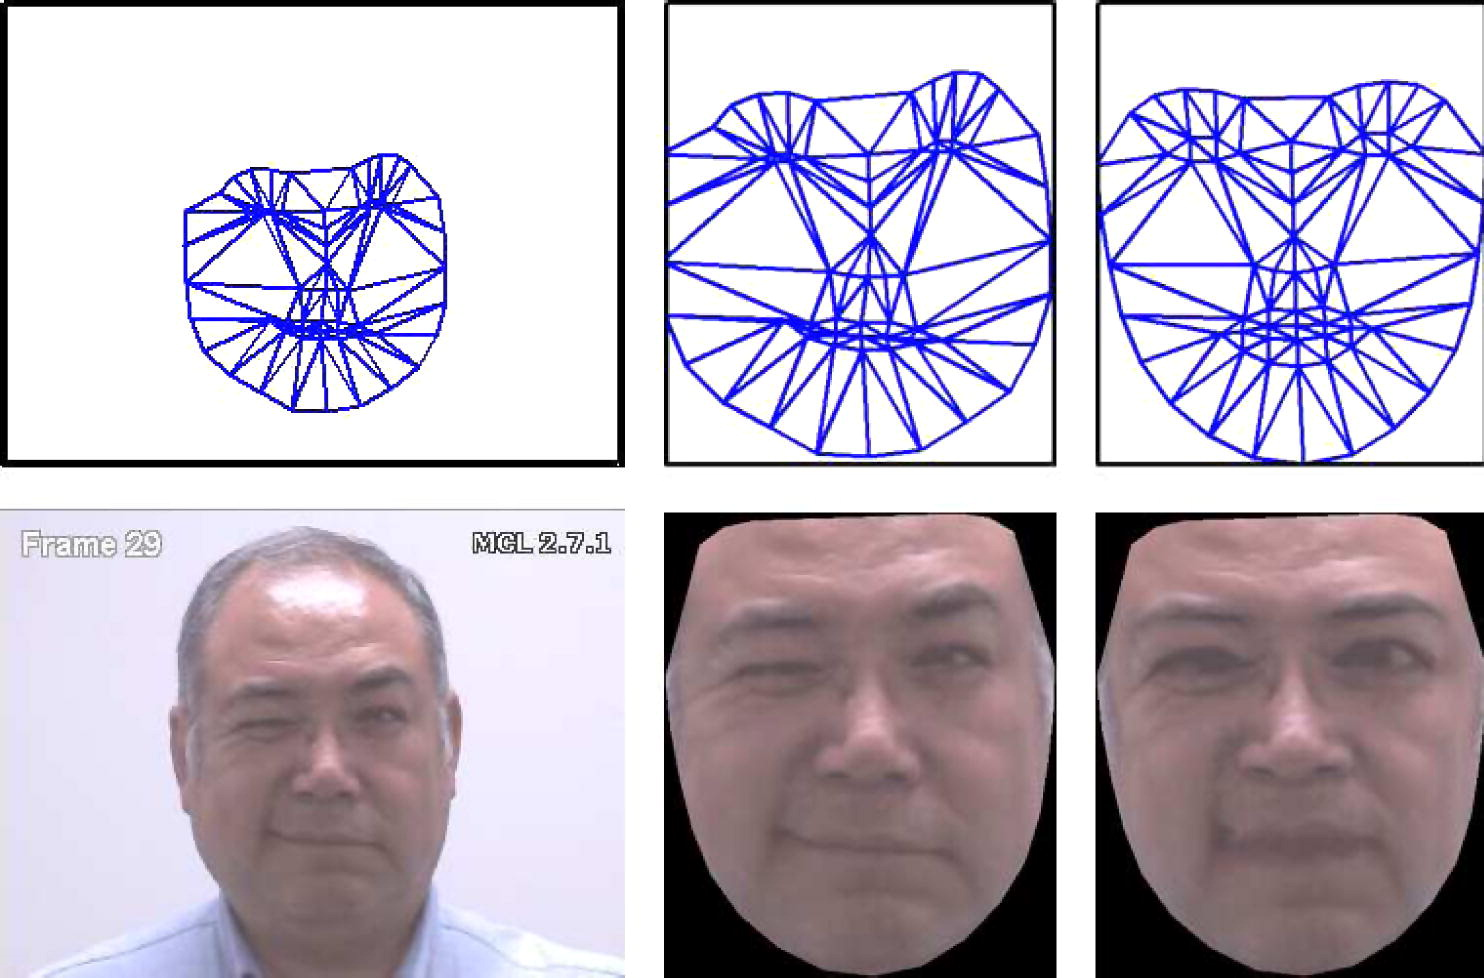
\includegraphics[width=0.7\textwidth]{C-APP_Example}
				\end{center}
				\caption{
					Example of image representations.
					Top row: Left, triangulation of raw landmarks. Middle, Procrustes aligned shape. Right, mean shape.
					Bottom row: Left, raw image. Middle, \textbf{S-APP}. Right, \textbf{C-APP}.
					Figure taken from \cite{Ashraf2009}.
					}
				\label{fig:app_strategies}
			\end{figure}

			A comparison of the two strategies is shown in Figure \ref{fig:app_strategies}.
			As \cite{Ashraf2009} rightly notes, it would seem that \textbf{C-APP} removes too much variation, eg. in the case of an eye closure as shown in Figure \ref{fig:app_strategies}.
			The case is though that \textbf{C-APP} preserves the most important part of this action, because the wrinkles around the eye is still very clear.
			These serve to distinguish between a \emph{twitch} as a result of pain and a regular blink, which does not result in these wrinkles.
			This distinction is a common cause for false positives in a pain recognition system.
			Further, the supposed lost information is conserved if the shape data and appearance is used together.

			In this project the \textbf{C-APP} representation is used.

			\paragraph{Implementing Image Warping} % (fold)
				\label{par:implementing_image_warping}
				The non-rigid warp of the facial appearance to the mean shape is done with at piecewise affine transformation.
				This means segmenting the face into triangles and the for each triangle warping the pixels inside to the corresponding triangle in the reference mean shape.
				The procedure is implemented as follows:
				\footnote{
					This is a general description of the implemented method. 
					For full MATLAB implementation see files \texttt{WarpImagesToMeanBatch.m} and \texttt{warpAppToMeanShape.m} in Appendix {\ref{sec:code}}
					}
				\begin{enumerate}
					\item
					The landmark points of the mean face shape needs to be put into a graph that connects all vertices into triangles without overlapping edges.
					There exists many solutions for this problem, but by making a Delauney triangulation, one can find the single solution that maximizes the smallest angle in all the triangles.
					This solution tends to avoid \emph{skinny} triangles and is a good fit for this application.

					The Delauney triangulation is made using MATALB's \texttt{delaunayTriangulation} function.
					It takes a set of points as input and returns a \emph{triangulation} object, which contain information about which vertices are connected in triangles (also called a \emph{Connectivity List}), and methods to determine in which triangle a certain point is inside.

					\item
					\emph{objectPixels} is determined by evaluating which pixel position is not inside any triangle of the Delauney triangulation of the mean shape.
					This results in a matrix of xy-coordinates, one row for each pixel.

					\item
					For each frame:
					\begin{enumerate}[label=\Roman*.]
						\item
						The image is loaded into MATLAB, converted to gray scale to conserve memory and converted to double-precision form int8 to facilitate calculation.

						\item 
						A new \emph{triangulation} object is then created using the connectivity list of the Delauney triangulation of the mean shape and the facial landmark points.
						This new triangulation is not an optimal Delauney triangulation.
						Instead it is a triangulation of the point in the frame where the triangle connections correspond to that of the Delauney triangulation of the mean shape.

						\item
						For each triangle in the Delauney triangulation of the mean shape:
						\begin{enumerate}[label=\roman*.]
							\item 
							An affine transformation matrix $\textbf{A}$, from the triangle to the correspond triangle in the new triangulation is calculated.
							\begin{equation}
								\label{eq:trans_mat} 
								\textbf{A} = 
								\begin{bmatrix}
									x_{a1} 	& x_{b1}	& x_{c1} \\
									y_{a1}	& y_{b1} 	& y_{c1} \\
									1 		& 1 		& 1
								\end{bmatrix}
								\bigg/
								\begin{bmatrix}
									x_{a2} 	& x_{b2}	& x_{c2} \\
									y_{a2}	& y_{b2} 	& y_{c2} \\
									1 		& 1 		& 1
								\end{bmatrix}
								=
								\begin{bmatrix}
									* & * & 0 \\
									* & * & 0 \\
									* & * & 1
								\end{bmatrix}
							\end{equation}
							In (\ref{eq:trans_mat}) $x_{a1}$, $x_{b1}$ and $x_{c1}$ is understood to be the x-coordinates of point $a$, $b$ and $c$, respectively, in the reference triangle.
							Likewise $y_{a2}$, $y_{b2}$ and $y_{c2}$ is the y-coordinates of point $a$, $b$ and $c$, respectively, in the corresponding triangle.

							\item
							The transformation matrix $\textbf{A}$ is then used to create a MATLAB \emph{transformationObject} using the \texttt{affine2d} function.
							This object has methods for handling the mapping of pixel positions with the affine warp.
						\end{enumerate}

						\item
						Then for each pixel position inside the new triangulation, the new pixel position is calculated using the appropriate \emph{transformationObject} and is stored along with its intensity.

						\item
						An interpolation has to be made to map the decimal coordinate value of the warped pixels to the integer grid of an image.
						This is done by making a MATLAB \emph{scatterdInterpolant} object.
						This takes all the decimal value positions and intensities of the warped pixel.
						You then define with interpolation method it is to use.
						In the project a \emph{linear} interpolation is used.

						\item
						The \emph{scatterdInterpolant} object can then be evaluated at all the coordinates of \emph{objectPixels} to output a vector of gray scale pixel intensities.
						
					\end{enumerate}

					\item
					It can happen that an error occurs when trying to calculate the transformation matrix $\textbf{A}$.
					This is typically due to excessive rotation/tilting of the subjects head, causing the matrix division to be impossible.
					In this case the error is simply logged and the script moves on to the next frame.
					The number of frames for which errors occur are around a couple hundred out of over 48000 frames.
					They are therefore deemed negligible and are omitted in further training and test.

				\end{enumerate}

			% subsubsection appearance_data (end)

		\subsubsection{Combining Data} % (fold)
			\label{ssub:combining_data}
			With the two datasets described in Sections \ref{ssub:shape_data} and \ref{ssub:appearance_data} above, it is possible to make, in total, three datasets, excluding the case of no data.
			That is:
			\begin{enumerate}
				\item
				\textbf{S-PTS}: 
				Only the Procrustes aligned shape data.
				This data is a vector $\textbf{s}_n$ stacking the 66 x-coordinates atop the 66 y-coordinates, resulting in a 132 dimensional feature space.

				\item
				\textbf{C-APP}:
				Only the shape normalized \emph{canonical} appearance.
				This data is a vector $\textbf{a}_0$ of 11646 dimensions that represent the pixel intensities at the coordinates listed in \emph{objectPixels}.

				\item
				\textbf{S-PTS + C-APP}:
				A combination of the shape and appearance data.
				The appearance data vector is stacked on top of the shape data vector to form a 11778 dimensional feature vector
				\begin{equation}
					\textbf{x}_{SPTS+CAPP} = 
						[\textbf{a}_0\ \textbf{s}_n] 
						\in \mathbb{R}^{11778}
				\end{equation}

			\end{enumerate}

			These datasets will then be used in the experiments of Sections \ref{sub:experiment_1_recognizing_facs_action_units} and \ref{sub:experiment_2_detecting_pain_in_faces} below.
			
			% subsubsection combining_data (end)
		
		% subsection data_pre_processing_and_feature_extraction (end)

	\subsection{Experiment 1: Recognizing FACS Action Units} % (fold)
		\label{sub:experiment_1_recognizing_facs_action_units}
		% Something about balanced examples
		\subsubsection{Purpose and Method} % (fold)
			\label{ssub:purpose_and_method_ex1}
			The purpose of this experiment is to see how well a linear SVM can be trained to recognize FACS Action Units from the data described in Section \ref{sub:data_pre_processing_and_feature_extraction}.
			The way this will be tested is by training a SVM using data from most of the subjects, and then validating against data from one or more other subjects that are not in the training set.
			The plan was initially to train a binary SVM for each FACS AU and do leave-one-subject-out cross validation on all subjects.
			This, however, was not possible for the following reasons
			\begin{enumerate}
				\item
				No one subject presents all the FACS Action Units relevant to the PSPI-score.
				Therefore validating all the classifiers against one control subject is not possible.

				\item
				The time is takes to train the 10 SVMs varies between 2 to 6 hours, depending on which dataset is used.
				Therefore it was not possible for me, within the time frame I have available, to do exhaustive cross-validating.
			\end{enumerate}

			The solution to this was to do the following:
			\footnote{See full MATLAB implementation in Appendix \ref{sec:code}: \texttt{compareSVMscore.m}}
			\begin{itemize}
				\item
				Select two subjects to be used as controls for validation, so that examples of all FACS AUs are present in both the training and validation set.
				I chose subjects 1 and 8 to be in the validation set.
				The rest are in the training set.

				\item
				For each FACS AU a set of training data was formed by taking all the positive examples in the training set and an equal number of randomly selected negative examples from training set.
				This ensured a uniform prior probability, and reduced the amount of data that was used, improving training time.

				\item
				The classifiers where trained using LIBSVM \cite{CC01a} in MATLAB.
				The implementation did not utilize the 6-core CPU very well, so the training was done in parallel using MATLABs \texttt{parfor} loops, with each SVM training on a separate thread, 6 at a time.

				\item
				The classifiers were evaluated by calculating the Receiver Operating Characteristics (ROC) Area Under the Curve (AUC).
				This relates the rate of True Positives (TP) to the rate of False Positives (FP) over a range of sensitivities, giving an easily comparable result between 0 and 1.

			\end{itemize}

			% subsubsection purpose_and_method (end)

		\subsubsection{Results} % (fold)
			\label{ssub:results_ex1}

			\paragraph{Recognizing FACS AUs with \textbf{S-PTS} data} % (fold)
				\label{par:recognizing_facs_aus_with_s-pts}
				\begin{figure}[H]
					\begin{center}
						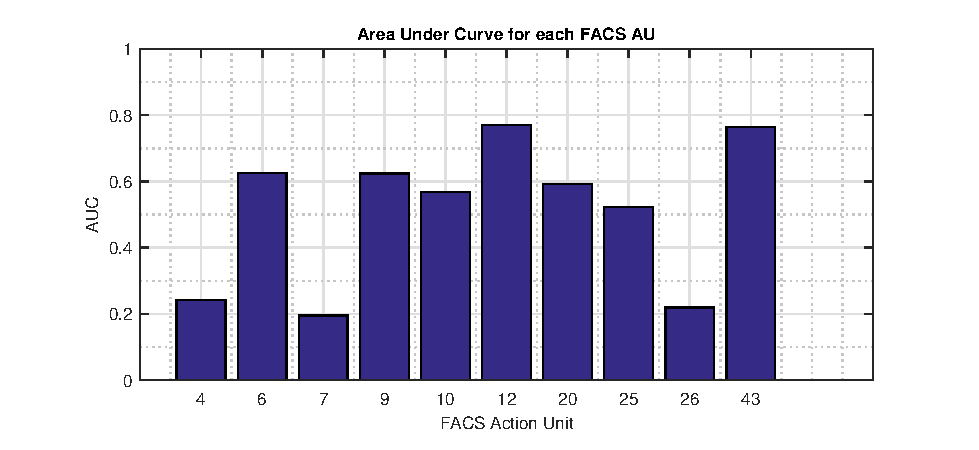
\includegraphics[]{FACS_AUC_PTS.eps}
					\end{center}
					\caption{
						AUC for \textbf{S-PTS} tested on subjects 1 and 8.
						SVM Trained on remaining subjects
						}
					\label{fig:spts_auc}
				\end{figure}
				
				% paragraph recognizing_facs_aus_with_s-pts (end)

			\paragraph{Recognizing FACS AUs with \textbf{C-APP} data} % (fold)
				\label{par:recognizing_facs_aus_with_c_app_data}
				\begin{figure}[H]
					\begin{center}
						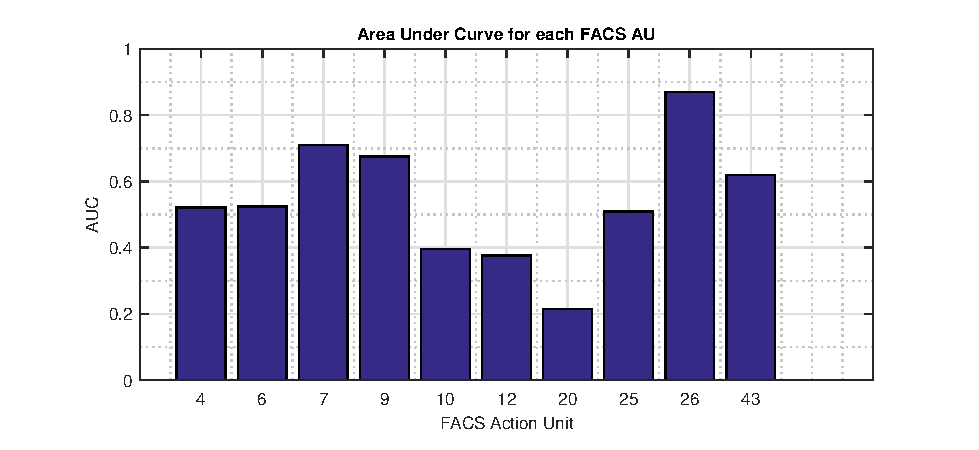
\includegraphics[]{FACS_AUC_App.eps}
					\end{center}
					\caption{
						AUC for \textbf{C-APP} tested on subjects 1 and 8.
						SVM Trained on remaining subjects
						}
					\label{fig:capp_auc}
				\end{figure}

			\paragraph{Recognizing FACS AUs with \textbf{S-PTS} + \textbf{C-APP} data} % (fold)
				\label{par:recognizing_facs_aus_with_s_pts_c_app_data}
				\begin{figure}[H]
					\begin{center}
						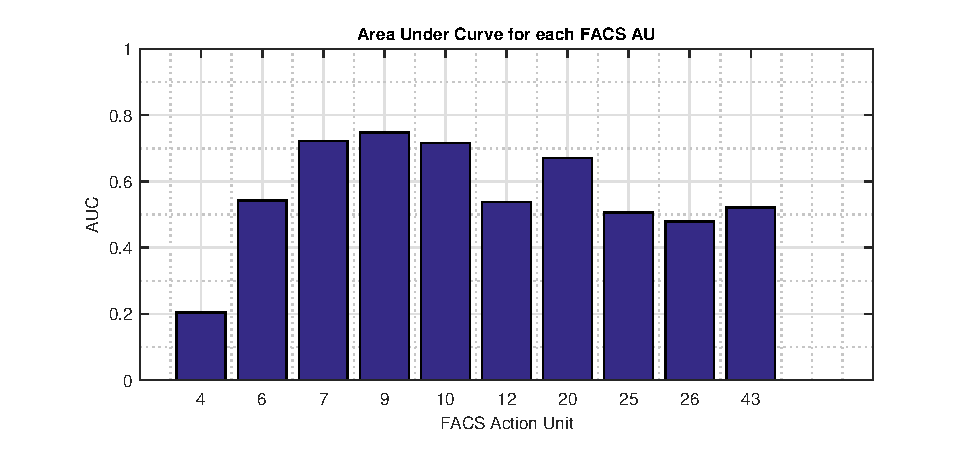
\includegraphics[]{FACS_AUC_Full.eps}
					\end{center}
					\caption{
						AUC for \textbf{S-PTS} + \textbf{C-APP} tested on subjects 1 and 8.
						SVM Trained on remaining subjects
						}
					\label{fig:full_auc}
				\end{figure}
				
				% paragraph recognizing_facs_aus_with_s_pts_c_app_data (end)
			
			% subsubsection results (end)
		
		% subsection experiment_1_recognizing_facs_action_units (end)

	\subsection{Experiment 2: Detecting Pain in faces} % (fold)
		\label{sub:experiment_2_detecting_pain_in_faces}
		\subsubsection{Purpose and Method} % (fold)
			\label{ssub:purpose_and_method_ex2}
			This experiment is very similar to Experiment 1 (See Section \ref{ssub:experiment_1}), in both purpose and method.
			Again a SVM is trained to classify based on the datasets described in Section \ref{sub:data_pre_processing_and_feature_extraction}.
			The difference here is that in stead of training to detect individual FACS AUs, the SVMs are trained to detect pain, in the form of the PSPI-score.
			\footnote{See full MATLAB implementation in Appendix \ref{sec:code}: \texttt{compareSVMscorePain.m}}
			
			% subsubsection purpose_and_method (end)


		\subsubsection{Results} % (fold)
			\label{ssub:results_ex2}
			\begin{figure}[H]
				\begin{center}
					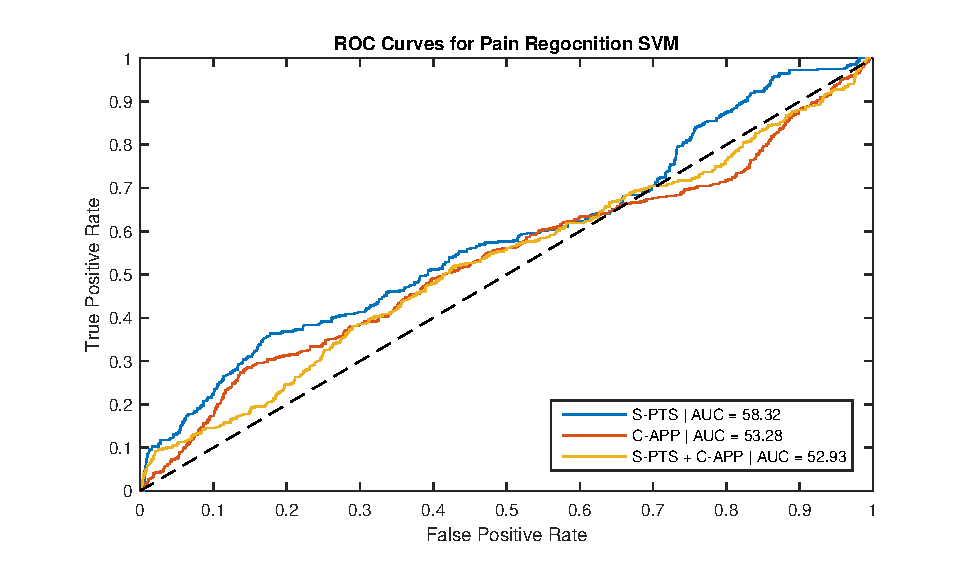
\includegraphics[]{PainAUC.eps}
				\end{center}
				\caption{
					Receiver Operating Characteristics curve for the SVMs trained on each data set.\\
					Area Under the Curve (AUC) given in percent.
					}
				\label{fig:pain_auc}
			\end{figure}
				
			% subsubsection results (end)
		
		% subsection experiment_2_detecting_pain_in_faces (end)

	\subsection{Discussion} % (fold)
		\label{sub:discussion}
		\subsubsection{Experiment 1} % (fold)
			\label{ssub:experiment_1}
			Comparing the results of this experiment to those of \cite{Lucey2011}, I have not been able to reach the same levels of performance.
			They see AUCs above random ($50\%$) for all AUs and all datasets.
			I only see a significant increase over random in for some AU with some datasets, and for some they do not even achieve that.

			There are however some similarities.
			Like \cite{Lucey2011} I find that the different data representations have complementary strengths and weaknesses, meaning that some Action Units are better described by shape variation, and some are better described by variation in appearance.
			I also see that overall performance evens out for the combined dataset, and that AUs that are strongly detected with either shape or appearance data do not necessarily have a strong response with the combined dataset.

			There may be several reasons for why my results differ so much from those of \cite{Lucey2011}.
			In my experiments the data is converted to gray scale.
			This is done to reduce the complexity of implementation and the amount of data that needs to be processed and hence processing time.
			It would seem that they used to full color images, although it does not say explicitly in the article.
			It may very well be that to much information is lost in converting to gray scale, and that this adversely affects performance.

			As the authors also note, there is a good portion of the samples where out of plane motion is significant.
			In the scope of this project it has not been possible for me to deal with this, which means that these will likely have interfered with the performance of the classifier, although in what way and to what extent I cannot say say with certainty.
			A test could be to manually exclude sequences where the subject moves excessively.

			In general there is a problem of availability of data.
			As noted in Section \ref{ssub:problems_with_using_the_unbc_database}, although the amount samples is large (> 48000) the amount of positive samples is comparatively low (< 8500), most of which are of low intensity.
			This means that amount of available training examples compared to the dimensionality of the data makes it hard to train a good model, especially for the very high dimensional \textbf{C-APP} and \textbf{S-PTS} + \textbf{C-APP} datasets.
			
			% subsubsection experiment_1 (end)
		
		\subsubsection{Experiment 2} % (fold)
			\label{ssub:experiment_2}
			The results of this experiment show that with this implementation it is not possible to detect pain with a certainty significantly greater than random.
			This is disappointing since \cite{Lucey2011} and subsequent authors have seen promising results with this approach.

			I believe that many of the same factors as those described in Section \ref{ssub:experiment_1} above are to blame for these results.
			That being said, I cannot say for sure that there are no errors in my implementation, as there are simply no more time in this project for further experimentation.			

			% subsubsection experiment_2 (end)

		% subsection discussion (end)

	% section normalized_appearance_and_shape_method_using_svm (end)

\end{document}